\documentclass[12pt]{article}
\usepackage[utf8]{inputenc,graphicx, booktabs, array} % Required for inserting images
\usepackage[paperheight=10.75in,paperwidth=8.25in,margin=1in,heightrounde]{geometry}
\usepackage[british]{babel}
\usepackage{indentfirst, amsmath, mathtools}
\usepackage[euler]{textgreek}
\usepackage{amssymb}
\linespread{1.5}
\title{Prírodovedecká fakulta Univerzity Karlovej \\ 
\Large Katedra aplikovanej geoinformatiky a kartografie}
\date{}

\begin{document}

\maketitle
\vspace*{-2cm}
\begin{center}

\includegraphics[scale=0.4]{latex/images/logo.png} 
\end{center}

\begin{center}
\textbf {Algoritmy počítačovej kartografie}\\
\textit{Zadanie č. 3: 	Digitálny model terénu a jeho analýza}\\
\vspace*{2cm}

\author {Bc. Filip Kradijan Seider\\Bc. Peter Dúbrava} \\
\date {2023/2024}
\\\LaTeX\
\end{center}
\thispagestyle{empty}

\newpage
\section*{Zadanie}\\
\noindent  Vstup: množina $P = \{p_1,..., p_n $\}, $p_i = \{x_i, y_i, z_i\}$. \\
Výstup: polyedrický DMT nad množinou P reprezentovaný obrysmi, doplnený vizualizáciou sklonu trojuholníkov a ich expozíciou.\par
 Na vytvorenie 2D Delaunayovej triangulácie nad množinou P vstupných bodov použite metódu inkrementálnej konštrukcie. Ako vstupné údaje použite existujúce geodetické údaje (aspoň 300 bodov) alebo navrhnite algoritmus na vytvorenie syntetických vstupných údajov reprezentujúcich významné tvary reliéfu (hromada, údolie, odpočinok, hrebeň, ...).\par
Vhodne vizualizujte súbory vstupných bodov vrátane nižšie uvedených výstupov. Implementujte grafické rozhranie pomocou rámca QT. Implementujte dynamické dátové štruktúry pomocou STL.\par
Nad výslednou trianguláciou vytvorte polyedrický digitálny model terénu. Potom vykonajte nasledujúce analýzy:
\begin{itemize}
    \item Pomocou lineárnej interpolácie vygenerujte obrysy s určeným krokom a v určenom intervale, vykonajte
ich vizualizáciu s rozlíšením zvýraznených kontúr.
    \item Analyzujte sklon digitálneho modelu terénu, vizualizujte jednotlivé trojuholníky podľa ich sklonu.
    \item Analyzovať expozíciu digitálneho modelu terénu, vizualizovať jednotlivé trojuholníky v závislosti od ich expozície voči svetovým stranám.
\end{itemize} \par
Vyhodnoťte výsledný digitálny model terénu z kartografického hľadiska, zamyslite sa nad slabými stránkami algoritmu založeného na 2D Delaunayovej triangulácii. V ktorých situáciách (rôzne tvary terénu) neposkytne vhodné výsledky? Graficky znázornite tieto situácie.\\\\\par
Vyhodnoťte výsledný digitálny model terénu z kartografického hľadiska, zamyslite sa nad slabými stránkami algoritmu založeného na 2D Delaunayovej triangulácii. V ktorých situáciách (rôzne tvary terénu) neposkytne vhodné výsledky? Graficky znázornite tieto situácie.\par
Vyhodnoťte výkonnosť algoritmu vrátane príkladov aspoň na 3 strany A4. \\\\\\\\
\begin{table}[htbp]
    \centering  
    \footnotesize
    \begin{tabular}{m{12cm}c}
        \toprule 
        \bfseries Úloha & \bfseries Hodnotenie \\ 
        \midrule 
        Delaunay triangulácia, polyedrický model terénu.& 10b \\
        Konštrukcia vrstevníc, analýza sklonu a expozície& 10b \\
        \bottomrule 
        \bfseries Spolu & \bfseries 20b
    \end{tabular}
\end{table}
\newpage
\section*{Problematika}
Realistické zobrazenie 3D povrchu Zeme je náročné, pretože ide o nepravidelný a členitý objekt. Niektoré miesta sú hladké, iné ostré, čo spôsobuje problémy pri ich aproximácii. Digitálny model terénu (DMT) je program na popis terénu v 3D. Terén je rozdelený na menšie plôšky, ktoré môžu byť aj zakrivené. Najčastejšie sa používajú plochy opísateľné polynomickými funkciami, ktoré plynulo na seba nadväzujú, aby bola zaručená spojitosť derivácií do určitého rádu. Tento proces prináša mnohé teoretické problémy, hlavne matematického charakteru (Vaníček 2024).\par

 V geopriestorovej analýze sú digitálne modely kľúčové pre pochopenie povrchu Zeme. Často sa ale stretneme aj s inými typmi modelov. Zatiaľ čo DTM sa zameriava na výšku holého povrchu Zeme bez povrchových objektov, tak DMR (digitálny model reliéfu) zachytávajú výškové údaje prírodných aj človekom vytvorených objektov (vegetácia, budovy). DMR sa používajú pri urbanistickom plánovaní, solárnom hodnotení a plánovaní sietí. DTM pomáhajú pri štúdiách povodia, erózie pôdy a hodnotení rizika záplav. Voľba správneho modelu závisí od toho, či projekt zahŕňa umelé a prírodné štruktúry alebo iba terén (Nordansjö, 2024).




\par
Podľa Bayera (2008) sa môže DTM deliť na naledujúce modely:
\begin{itemize}
    \item Polyedricky model sa skladá z nepravidelných trojuholníkov, ktoré pokrývajú celé územie a majú spooločnú najvzššiu hranu. Na jeho tvorbu sa najčastejšie vzužíva triangulačnýý algoritmus.
    \item Rastrový, alebo aj gridový model je tvorený pravidelnou štvorcovou sieťou, ktorú je možné rozdeliť aj na trojuholníky. Táto metóda sa neprispôsobuje terénu, čo môže v niektorých jeho miestach spôsobovať nadbztok, či nedostatok bodov. 
    \item  Plátový model je z estetického hladiska lepší ako predchádyajúce dva modely, avšak náročnejší. Medzi susednými plochami vytvára hladké prechody s využitím  plátov. Tieto pláty možu mať trojuholníkový, ale aj štvorcový tvar.
\end{itemize} \par

\subsection*{Tvorba digitálne modelu terénu}
Postup tvorby DTM prebieha v niekoľkých fázach, ako napríklad získavanie vstupných dát a vytvorenie triangulácie z povinných hrán. Kvalita vytvoreného DTM závisí od rozmiestnenia bodov (ideálne v miestach so zmenou sklonu a minimalizovaním veľkých plôch bez bodov), typu triangulačného algortizmu (\textit{Delaunayho, Minimum Weight}) a plátov (najlepšie výsledky majú Beziérové kubické pláty), či aj od presnosti vstupných dát (Bayer, 2008). \par
Polyedricky typ DMT využíva sieť trojuholníkových plôch vytvorenú trianguláciou. Triangulačný algoritmus prepája trojice vrcholov do roviny v $\mathbb{R}$3, čím vzniká nepravidelný mnohosten (polyéder), ktorý sa prispôsobuje terénu. TIN (\textit{Triangular Irregular Network}) je efektívny pri heterogénnych povrchov, pretože oblasti s väčšou variabilitou sú uložené podrobnejšie pomocou väčšieho počtu dátových bodov a homogénne oblasti sú uložené pomocou mála dátových bodov. Inými slovami, TIN môže byť podrobnejší tam, kde je povrch zložitý (s vysokou variabilitou) použitím menších plôch, a menej podrobný tam, kde je povrch homogénnejší použitím väčších plôch (Brůha, 2016; Lim \& Pilesjö, 2022). 

\subsubsection*{Delaunayho triangulácia}
Delaunayova triangulácia (DT)je jednou z najpopulárnejších a najčastejšie používaných metód na generovanie trojuholníkových sietí. Posledncýh 20 rokov bola intenzívne študovanáv, hoci základy boli položené už začiatkom 20. storočia (Voronoi, Delaunay) Výsledné trojuhelníky sa spomedzi všetkých známich triangulácií najviac približujú rovnostranným (Maur, 2002). Bayer vo svojej knihe uvádza nasledujúce vlastosti: 
\begin{itemize}
    \item Vo vnútri žiadnej kružnice z opísaných trojúhelníkov  $t_j \in $  DT neleží žiaden z bodov množiny P.

    \item DT maximalizuje minimálny úhol v $\forall$ t, avšak DT neminimalizuje maximálny uhol v trojuholníku.
    \item DT je lokálne aj globálne optimalizovaný voči kritériu minimálneho úhla.
    \item DT je jednoznacná, pokiaľ žiadne štyri body neležia na kružnici, inak existuje viacero varian (dochádza k tomu hlavne pri pravidelnej sieti bodov).
\end{itemize}  \par
Existuje viacero priamych metód tvorby DT, avšak pre účely tohto cvičenia nás zaujíma iba inkrementálna konštrukcia so zložitosťou $(O(n^3))$. Túto metódu je možné využiť ako v 2D (kružnica), tak aj v 3D (sféra) a je založená na princípe postupného pridávania bodov. Dostaneme tak rovinu rozdelenú na tojuholníky, pri ktorých platí, že ľubovoľné dva trojuholníky majú spoločnú maximálne jednu hranu a zjednotením všetkých trojuholníkov sa vytvorí konvexný obal množiny bodov \textit{P} (Vaníček, 2010).\par
\begin{figure}[h]
    \centering
    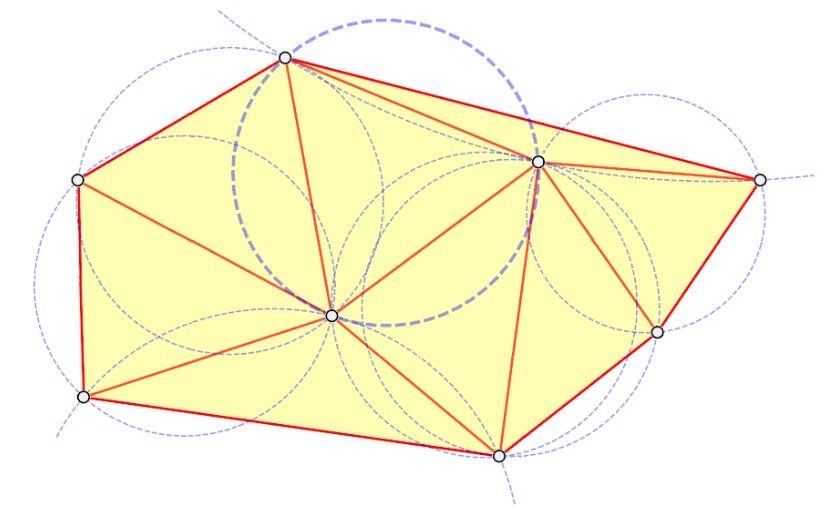
\includegraphics[width=0.8\linewidth]{latex/images/dt.jpg}
    \caption{Delaunay triangulácia (Bayer, 2024)}
    \label{fig:enter-label}
\end{figure}
Je daná množina bodov \textit{P}=\{$p_1, p_2, ...; p_n$\} v rovine $\mathbb{R}$2 a každý z bodov je reprezentovaný súradnicami \textit{x, y, z}. Vyberie sa jeden bod a následne sa ku nemu hľadá ďalší, podľa euklídovskej vziadelenosti najbližší bod. Vznikne tak prvá orientovaná Delaunayovská hrana \textit{e=\{$p_1, p_2$\}}. Ku hrane sa následne hľadá v jej ľavej polrovine \textit{e} Delaunay point $\bar{p}$ pomocou maximalizovania uhlov trojuholníka $\angle(p_1, p, p_2)$:
$$\bar{p} = arg \max\limits_{\forall p_i \in \sigma_L  (e)} \angle(p_1, p_i, p_2),\hspace{1cm}  p_i \in \sigma_I(e),$$ avšak pokiaľ takýto bod neexistuje, tak sa zmení orientácia hrany a proces sa opakuje. Do DT sa následne pridávajú hrany trojuholníka \textit{$\triangle(p_1, p_2, \b{p})$}: 
$$e_1 = (p_2,\bar{p}),\hspace{1cm}  e_2 = (\bar{p}, p_1).$$ \par
 Musia však pri tom spĺňať podmienku, že ich opačné orientácie sa nemôžu nachádzať v Active Edge List (AEL):

$$ e'_1 = (\bar{p}, p_2),\hspace{1cm}  e'_2 = ( p_1, \bar{p})$$.
Tento list obsahuje hrany, ku ktorým sa hľadajú Delaunay points a po vyprázdnení tohto zoznamu je vytvorená celá DT.
\subsection*{Analýza reliéfu}
Nad vytvoreným DTM je možné riešiť rôzne analytické operácie, či odvodiť ďalššie parametre. Medzi takéto operácie patrí hlavne tvorba vrstevníc potrebná pre hypsometriu. Ďalej je dôležitý sklon reliéfu pre potreby súvisiace s výskytom lavín, zosuvov a erózií, či expozícia reliéfu pre potreby poľnohospodárstva (Bayer) 
\subsubsection*{Tvorba vrstevníc}
Vrstevnice alebo izohypsy sú krivky spájajúce body s rovnakou nadmorskou výškou, pričom platí, že čím sú vrstevnice hustejšie, tým znázorňujú väčšie prevýšenie. Vrstevnice sú vytvorené lineárnym interpolačným algoritmom, vďaka tomu je rozostup vrstevnic medzi dvomi bodmi konštantný. Takýto výpočet je jednoduchý, ale úplne nevystihuje realitu. Tento algoritmus je založený na princípe analytickej geometrie. Dochádza ku hľadaniu priesečníku \bar{AB} medzi rovinou plátu \textit{T}$(p_1, p_2, p_3)$ určenej trojúhelníkom \textit{t} $\in$ DT a vodorovné roviny $\varrho$  s výškou \textit{h}. Tento proces sa opakuje nad  všetkými rovinami plátov \textit{t} (Bayer, 2008; Bayer, 2024). \par\newpage
Súradnice bodov A,B predstavujúcich priesečníky rovín, ktoré sa získajú na základe nasledujúcich vzťahov za využitia podobnosti trojuholníkov:
$$ x_a = \frac{x_3 - x_1}{z_3 - z_1}(z - z_1) + x_1,\hspace{1cm}  x_b = \frac{x_2 - x_1}{z_2 - z_1}(z - z_1) + x_1,$$
$$ y_a = \frac{y_3 - y_1}{z_3 - z_1}(z - z_1) + y_1,\hspace{1cm}  y_b = \frac{y_2 - y_1}{z_2 - z_1}(z - z_1) + y_1 $$
Overenie, či plocha $\varrho$ pretína stranu trojuholníka (p_i, p_{i+1}): $ \triangle z_i \triangle z_{i+1}<0$, kde $$\triangle z_i = z_i - z, \hspace{1cm}  \triangle z_{i+1} = z_{i+1} - z.$$


\subsubsection*{Sklonu reliéfu}
Sklon reliéfu je najpoužívanejší morfometrický ukazovateľ reliéfu. Sklon  možno definovať ako uhol, ktorý zviera dotyková rovina k danému bodu s horizontálnou rovinou, rovnobežnou s hladinou svetového oceána. Ďalšia možná definícia je  sklon reliéfu predstavuje zmenu nadmorských výšok v smere spádovej krivky. Vyjadruje sa v stupňoch (Kubínsky, 2024). \par
Podľa Bayera (2024) je výpočet sklonu vykonaný na každom trojuholníku za pomoci vektoru maximálneho spádu (gradient). Pri tom platí, že rovnica  roviny $\varrho$ má tvar $\rho : ax + by + cz + d = 0$ a jej gradient  $\nabla f(x_0, y_0, z_0)$ funkcie $f(x, y, z) $ v bode $ p = [ \ x_0, y_0, z_0]\ $ je určený nasledujúcim vzťahom: $$\nabla f (x_0, y_0, z_0) = (\frac{\partial f }{ \partial x}(x_0), (\frac{\partial \rho }{ \partial y}(y_0),(\frac{\partial \rho }{ \partial z}(z_0))= (a, b, c)$$\par
Okrem roviny $\varrho$ sa tu nachádza aj vodorovná rovina $\pi$. Normálové vektori týchto rovín $n_1$ a $n_2$ sa následne podielajú na výpočte sklonu (odchýlka $\varphi$): $$
\varphi = \arccos \left( \frac{n_1 \cdot n_2}{\lVert n_1 \rVert \lVert n_2 \rVert} \right) = \arccos \left( \frac{c}{\lVert n_1 \rVert} \right),
$$
kde normálový vektor $n_2$ roviny $\pi$ sa považuje za jednotkový:
$$ n_1 = (a, b, c),\hspace{1cm} n_2 = (0, 0, 1).$$
\begin{figure}[h]
    \centering
    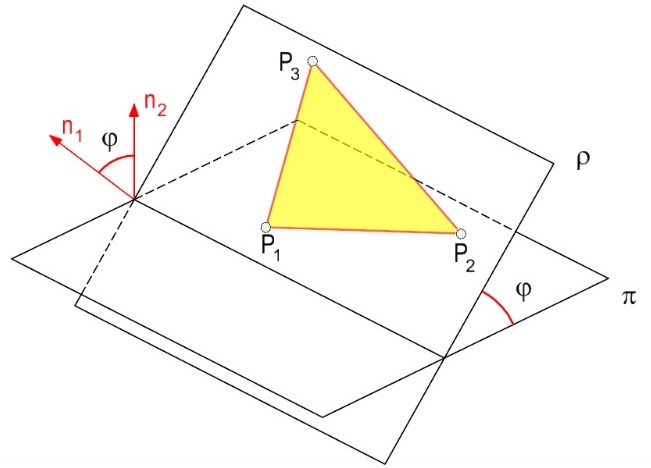
\includegraphics[width=0.8\linewidth]{latex/images/sklon.jpg}
    \caption{Sklom reliéfu (Bayer, 2024)}
    \label{fig:enter-label}
\end{figure}
\newpage
\subsubsection*{Expozície reliéfu}
Expozícia, alebo aj aspekt, slúži na vyjadrenie smeru, ktorým je povrch reliéfu orientovaný voči svetovým stranám. Je meraný v azimutoch od 0 do 360, pričom začína od severu (0°) v smere hodinových ručičiek. Určenie expozície zahŕňa vytvorenie izotangent, ktoré spájajú body s rovnakou orientáciou reliéfu (Dekan, 2022).
Bayer (2024) definuje orientáciu reliéfu ako azimut priemetu gradientu do roviny. Tento vektor $\vec{v}$ má nulovú zložku a je vyjazdrený nasledovne:
$$v = (\frac{\partial \rho }{ \partial x}(x_0), \frac{\partial \rho }{ \partial y}(y_0),0)=(a, b, 0).$$
Azimut A medzi vektorom $\vec{v}$ a osou \textit{y} je následne vypočítaný ako:
$$ A = arctan (\frac{a}{b}). $$ \par
Výpočet je potrebné spraviť pre každým trojuholník digitálne modelu a je potrebné byť obozretný pri správnom určovaní kvadrantu.
\newpage

\begin{figure}[h]
    \centering
    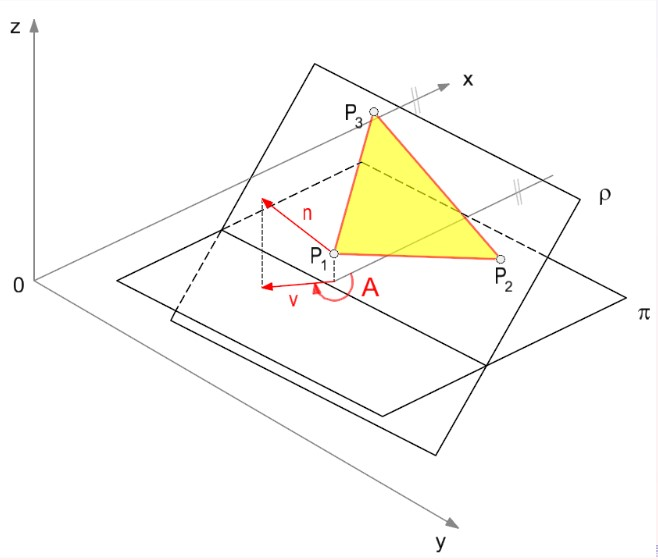
\includegraphics[width=0.8\linewidth]{latex/images/aspekt.jpg}
    \caption{Orientácia reliéfu (Bayer, 2024)}
    \label{fig:enter-label}
\end{figure}

\clearpage 
\section*{Implementácia}
Po priblížení problematiky a vysvetlení metód na jej riešenie je ďalším krokom v tomto zadaní tvorba užívateľského prostredia, v ktorom bude možné demonštrovať  degitálny model terénu. Tento model obsahuje lokality s odlišnými vlastnosťami.
\subsection*{Vstupné dáta}
Ako oblasť  záujmu sme si vybrali uzemie v okolí , ktoré sa vďaka svojej členitosti (vrcholy, chrbty, roviny, doliny) javilo ako najlepšie pre potreby tohoto zadania. Najprv bolo potrebné pre toto uzemie stiahnuť TIFF (zdroj: ÚGKK SR) obsahujúci informáciu o výške . Použili sme webovú aplikáciu ZBGIS a pre naše územie sme stiahli digitálny model reliéfu 5. Následne sme pre toto územie vytvorili náhodné body s minimálnym vzdialenosťou 300 m v aplikácii ArcGisPRO použitím funkcie \textit{Create random point}. Následne bolo potrebné spočítať pre tieto body súradnice x a y pomocou \textit{Calculate geometry atributes} a hodnoty výšok boli ku našim bodom priradené z TIFF vďaka funkcii \textit{Extract values to points}. Dostali sme tak 1000 nádodných bodov v súradnicovom sýstému EPSG:5514.
\begin{figure}[h]
    \centering
    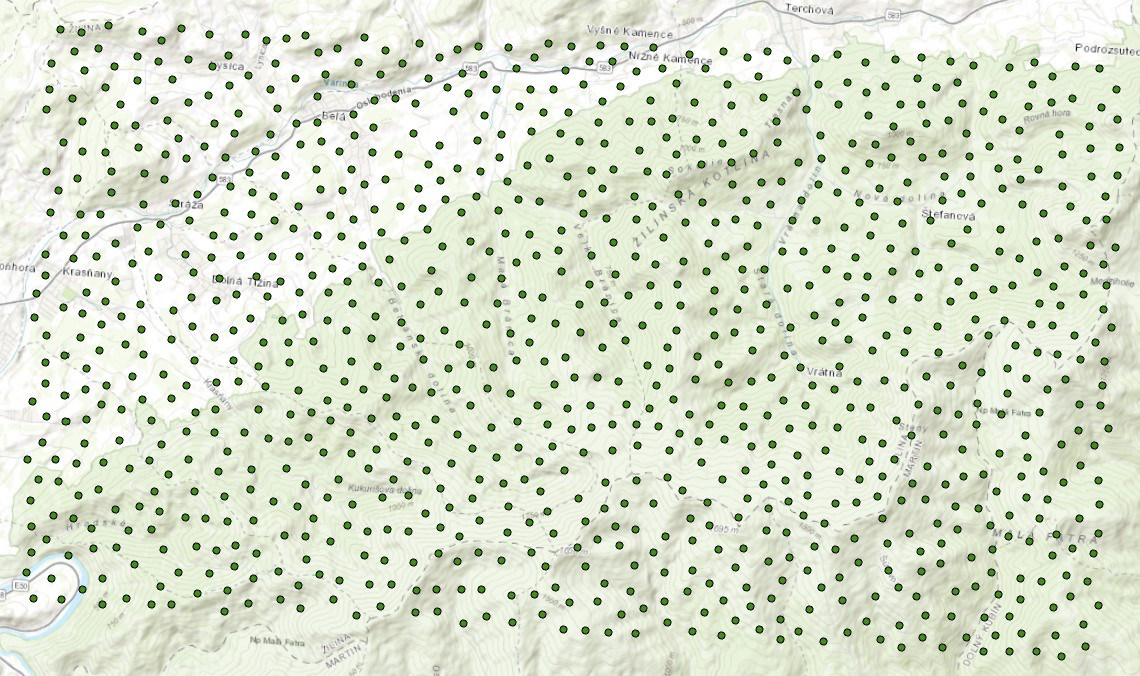
\includegraphics[width=0.8\linewidth]{latex/images/body.jpg}
    \caption{Množina vytvorených bodov nad územím}
    \label{fig:enter-label}
\end{figure}
 
\subsection*{Aplikácia}
Grafické užívateľské prostredie (GUI) aplikácie  pozostávalo z okna, lišty a panelu obsahujúceho ikony, ktoré bolo vytvorené za pomoci knižnice QT (v.4.6.1) a jeho funkcionalita bolo ďalej doplňovaná za pomoci programovacieho jazyka Python 3.11. Vďaka tomu bolo možné pre jednotlivé ikony pridať aj ich funkcie.
\begin{figure}[h]
    \centering
    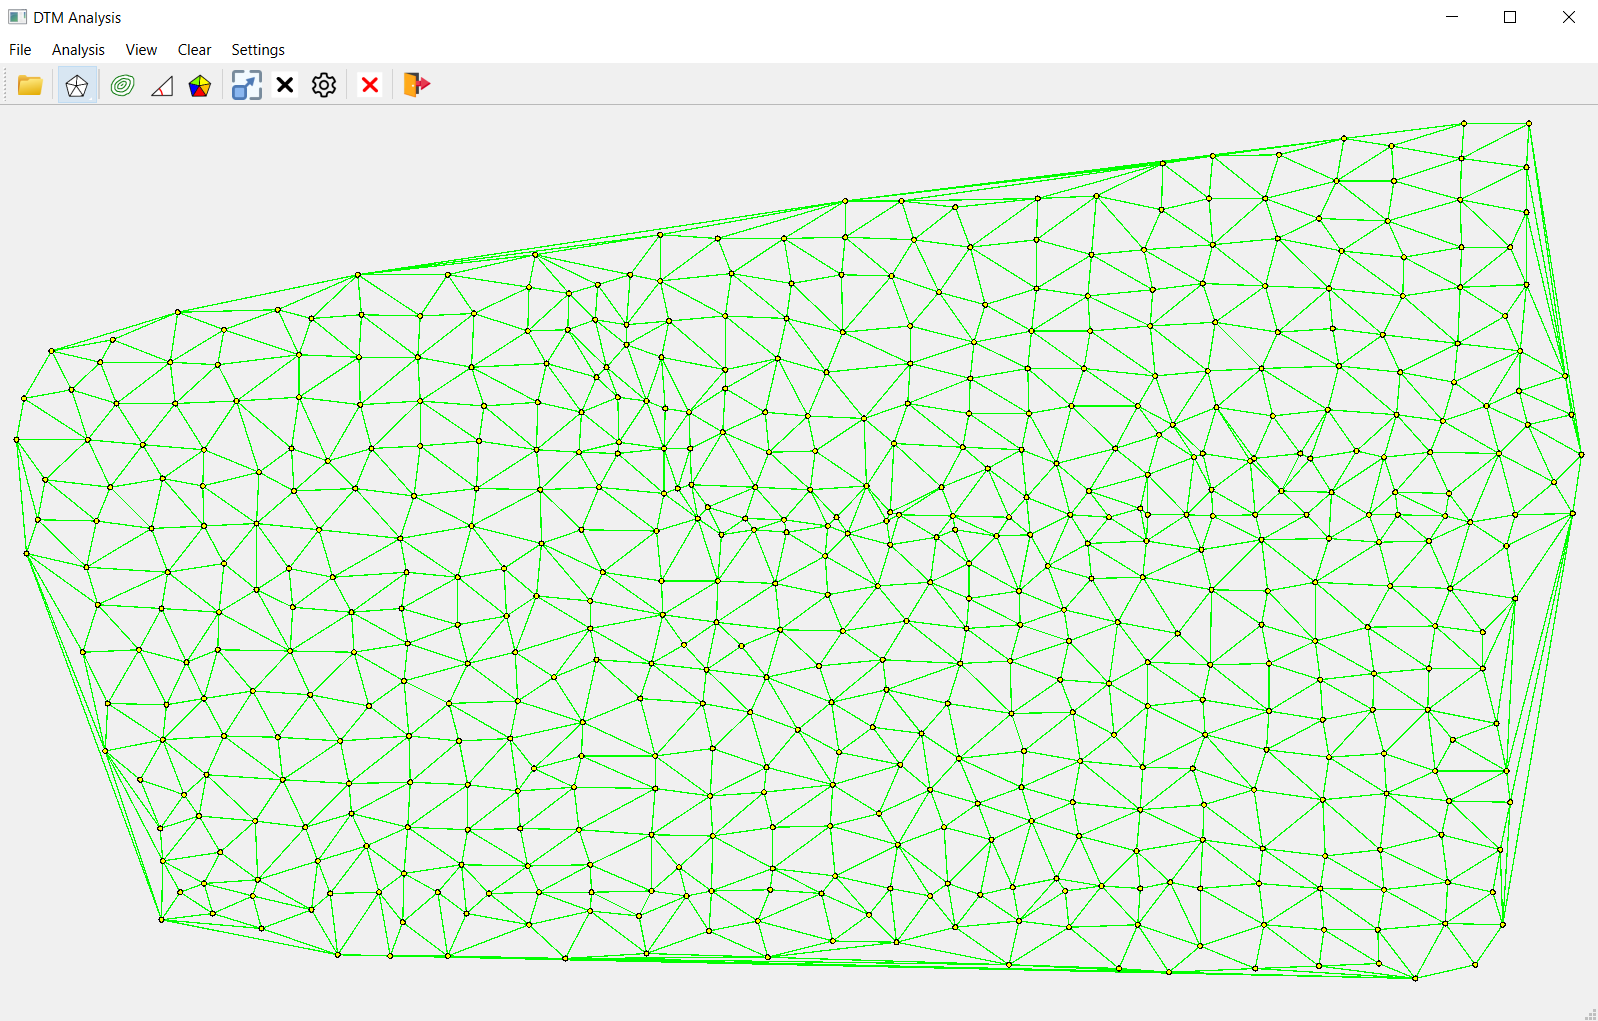
\includegraphics[width=0.7\linewidth]{latex/images/apk.png}
    \caption{Prostredie aplikácie}
    \label{fig:enter-label}
\end{figure}
\par Celkovo bolo použitých 10 ikon (obr. ), ktorých úlohou je urýchliť prácu používateľa, 
vďaka čomu nie je potrebné prechádzať lištu a hľadať jednotlivé procesy, ktoré by sme pri 
väčšej komplexnosti aplikácie mohli prehliadnuť.
\begin{figure}[h]
    \centering
    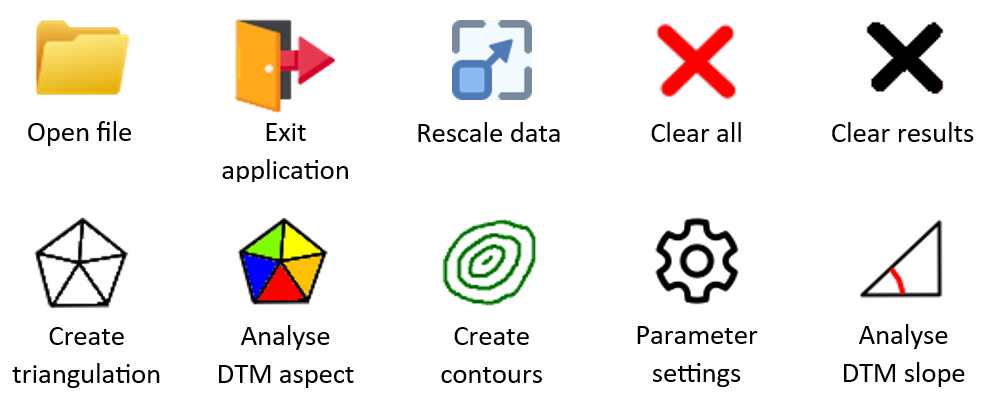
\includegraphics[width=0.7\linewidth]{latex/images/icons.png}
    \caption{Ikony použité v aplikácii}
    \label{fig:enter-label}
\end{figure}
\clearpage 
\section*{Dokumentácia}
\subsection*{Algorithms}
Trieda Algorithms je navrhnutá na vykonávanie série geometrických výpočtov a analýz súvisiacich s modelovaním terénu, najmä so zameraním na Delaunayovu trianguláciu, generovanie vrstevníc a analýzu sklonu a orientácie vytvorených trojuholníkov. 
\subsubsection*{get2LineAngle(p1: QPointF, p2: QPointF, p3: QPointF, p4: QPoint)F}
\noindent -vypočíta uhol medzi dvoma čiarami definovanými bodmi (p1, p2) a (p3, p4)
\subsubsection*{getNearestPoint(q: QPoint3DF, points: list[QPoint3DF])}
\noindent -nájde najbližší bod k bodu \textit{q} zo zoznamu points
\subsubsection*{twoPointDist(from\textunderscore p: QPoint3DF, to\textunderscore p: QPoint3DF)}
\noindent-Vráti vektorovú vzdialenosť medzi dvomi bodmi v súradniciach \textit{x} a \textit{y}.
\subsubsection*{getDelaunayPoint(start: QPoint3DF, end: QPoint3DF, points: list[QPoint3DF])}
\noindent-nájde optimálny Delaunayov bod pre úsečku
\subsubsection*{updateAEL(e: Edge, ael: list[Edge])}
\noindent-aktualizuje zoznam aktívnych hrán (AEL) pridaním alebo odstránením hrany
\subsubsection*{createDT(points: list[QPoint3DF])}
\noindent-vytvára Delaunayovu trianguláciu pomocou inkrementálnej metódy
\subsubsection*{getContourPoint(p1: QPoint3DF, p2: QPoint3DF, z: float)}
\noindent-vypočíta priesečník hrany trojuholníka s horizontálnou rovinou vo výške \textit{z}
\subsubsection*{createContourLines(dt: float, zmin: float, zmax: float, dz: float)}
\noindent-vytvára vrstevnicové línie z Delaunayovej triangulácie
\subsubsection*{computeSlope(p1: QPoint3DF, p2: QPoint3DF, p3: QPoint3DF)}
\noindent-vypočíta sklon trojuholníka
\subsubsection*{computeAspect(p1: QPoint3DF, p2: QPoint3DF, p3: QPoint3DF)}
\noindent-vypočíta aspekt (orientáciu) trojuholníka
\subsubsection*{normalsVectors(p1: QPoint3DF, p2: QPoint3DF, p3: QPoint3DF)}
\noindent-vypočíta normálový vektor trojuholníka
\subsubsection*{analyzeDTMSlope(dt: list[Edge])}
\noindent-analyzuje sklon každého trojuholníka v Delaunayovej triangulácii.
\subsubsection*{analyzeDTMAspect(dt: list[Edge])}
\noindent-analyzuje aspekt každého trojuholníka v Delaunayovej triangulácii.
\subsubsection*{sjtsk2Pixel(pnt: list, width: int, height: int, x\textunderscore min: float, x\textunderscore max: float, y\textunderscore min: float, y\textunderscore max: float)}
\noindent-konvertuje súradnice zo systému SJTSK na pixlové súradnice
\subsubsection*{uniquePerDim(points: list)}
\noindent-určí počet unikátnych súradníc na osiach \textit{x} a \textit{y}
\subsubsection*{rescale(points: list, dt: list, contours: list, slope: list, aspect: list, w: int, h: int)}
\noindent-na základe nových rozmerov zmení mierku všetkých dáta, aby sa zmestili do canvasu.

\subsubsection*{rescaledCoords(pnt: QPoint3DF, x\textunderscore min: float, y\textunderscore min: float, del\textunderscore pix\textunderscore x: int, del\textunderscore pix\textunderscore y: int, del\textunderscore data\textunderscore x: float, del\textunderscore data\textunderscore y: float}
\noindent- počíta reskalované súradnice pre metódu rescale().

\subsection*{Draw}
Táto trieda poskytuje komplexné funkcie pre vizualizáciu a interakciu s 3D bodovými mrakmi,  Delaunayovej triangulácie (DT), vrstevníc, sklonu a aspektu modelu. Obsahuje viacero funkcií typu \textit{get} a \textit{set}, ktoré slúžia pre prístup a nastavovanie dát so zobrazením. 
\subsubsection*{\textunderscore\textunderscore init\textunderscore \textunderscore(self, *args, **kwargs)}
\noindent-inicializuje widget a jeho vlastnosti. Nastaví zoznamy na ukladanie bodov, triangulácie, vrstevníc, sklonov a aspektov. Taktiež inicializuje príznaky pre rôzne možnosti zobrazenia (DT, vrstevnice, sklon, aspekt) 
\subsubsection*{mousePressEvent(self, e: QMouseEvent)}
\noindent-spracováva informácie stlačením myši. Získa \textit{x} a \textit{y} súradnice kurzora, vygeneruje náhodnú \textit{z} súradnicu (výšku), vytvorí nový 3D bod (QPoint3DF) a pridá ho do zoznamu points. Nakoniec spustí prekreslenie widgetu
\subsubsection*{messageBox(self, title: str, text: str)}
\noindent-zobrazí dialógové okno s určeným názvom a textom. To je užitočné pre poskytovanie spätnej väzby alebo informácií používateľovi.
\subsubsection*{paintEvent(self, e: QPaintEvent)}
\noindents-spracováva kreslenie widgetu. Používa objekt QPainter na kreslenie bodov, Delaunayovej triangulácie, vrstevníc, sklonov a aspektov podľa aktuálnych nastavení zobrazenia.
\subsubsection*{clearAll(self)}
\noindent-vymaže všetky dáta (body, DT, vrstevnice, sklony, aspekty) a prekreslí widget.
\subsubsection*{clearResults(self)}
\noindent-vymaže výsledky (DT, vrstevnice, sklony, aspekty), ale ponechá body nedotknuté a potom prekreslí widget.
\subsection*{Edge}
Trieda Edge poskytuje základné funkcie na reprezentáciu a manipuláciu hrán v 3D priestore.
\subsubsection*{\textunderscore\textunderscore init\textunderscore\textunderscore(self, start: QPoint3DF, end: QPoint3DF)}
\noindent-inicializuje objekt Edge s počiatočnými a koncovými bodmi. Tieto body sú typu QPoint3DF, čo znamená, že majú \textit{x, y} a \textit{z} súradnice
\subsubsection*{getStart(self)}
\noindent-vráti počiatočný bod hrany
\subsubsection*{getEnd(self)}
\noindent-vráti koncový bod hrany
\subsubsection*{changeOrientation(self)}
\noindent-vytvorí a vráti novú hranu s obrátenou orientáciou (t.j. počiatočný bod sa stane koncovým a koncový bod sa stane počiatočným).
\subsubsection*{\textunderscore\textunderscore  eq \textunderscore\textunderscore (self, other)}
\noindent-Porovnáva rovnosť dvoch hrán. Hrany sú rovnaké, ak majú rovnaký počiatočný a koncový bod.
\subsection*{IO}
Trieda pre načítanie a ukladanie dát. - Dialog na načítanie súboru prijíma iba súbory s príponami *.TXT, *.GeoJSON a *.JSON - Načíta súbory s formátovaním GeoJSON - Program predpokladá dáta v S-JTSK CRS (EPSG: 5514).
\subsubsection*{load(self, file: str, width: int, height: int)}
\noindent-načítava dáta zo zadaného súboru a prevádza ich do pixlových súradníc.
\subsection*{Ui \textunderscore MainWindow}
Vytvára užívateľské rozhranie a obsahuje metódy na ovládanie grafických funkcií aplikácie. 
viewDTClick(self), viewContourLinesClick(self), viewSlopeClick(self), viewAspectClick(self):
Umožňujú zapnúť alebo vypnúť zobrazenie rôznych vrstiev dát.
\subsubsection*{setupUi(self, MainWindow)}
\noindent-inicializuje užívateľské rozhranie pre hlavné okno aplikácie
\subsubsection*{openClick(self)}
\noindent-obsluhuje akciu otvorenia súboru a načítania bodov z daného súboru
\subsubsection*{createDTClick(self)}
\noindent-vytvára Delaunayovu trianguláciu zo súčasne načítaných bodov
\subsubsection*{createContourLinesClick(self)}
\noindent-vytvára kontúrové čiary z aktuálnej Delaunayovej triangulácie podľa zadaných parametrov
\subsubsection*{analyzeSlopeClick(self)}
\noindent-analyzuje svahy v aktuálnej Delaunayovej triangulácii
\subsubsection*{analyzeAspectClick(self)}
\noindent-analyzuje orientácie svahov v aktuálnej Delaunayovej triangulácii
\subsubsection*{clearClick(self)}
\noindent-vyčistí výsledky analýz zo zobrazovacej plochy
\subsubsection*{clearAllClick(self)}
\noindent-vyčistí všetky dáta zobrazené na zobrazovacej ploche
\subsubsection*{rescaleClick(self)}
\noindent-zmení mierku zobrazenia bodov podľa veľkosti aktuálneho okna aplikácie
\subsubsection*{setParameters(self)}
\noindent-zobrazuje dialógové okno pre nastavenie parametrov
\subsubsection*{close(self)}
\noindent-zatvára aplikáciu

\subsection*{QPoint3DF}
Trieda QPoint3DF rozširuje triedu QPointF o ďalšiu súradnicu Z. To je dôležité pre operácie, ktoré prebiehajú v 3D priestore, ako je napríklad naša Delaunayova triangulácia.
\subsubsection*{\textunderscore \textunderscore init\textunderscore \textunderscore (self, x: float, y: float, z: float)}
\noindent-konštruktor triedy inicializuje nový objekt bodu s danými x, y, a z-koordinátami.

\subsubsection*{getZ(self)}
\noindent-metóda vráti hodnotu z-koordináty daného bodu.
\subsection*{ Ui\textunderscore Settings}
Trieda Ui\textunderscore Settings vytvára pop-up okno, ktoré umožňuje užívateľovi zadať minimálnu a maximálnu výšku vrstevníc, ako aj interval medzi nimi.
\subsubsection*{setupUi(self, Settings)}
\noindent-nastaví užívateľské rozhranie pre dialógové okno nastavení. Definuje tlačidlovú lištu pre potvrdenie alebo zrušenie nastavení a skupinu prvkov pre nastavenie parametrov kontúrových línií.
\subsubsection*{retranslateUi(self, Settings)}
\noindent-metóda preloží texty zobrazené v dialógovom okne nastavení
\subsection*{Triangle}
Definuje trojuholník v 2D priestore. Trojuholník je určený tromi bodmi (vrcholmi) \textit{p1, p2} a \textit{p3}. Vracia sklon a expozíciu trojuholníkov.
\subsubsection*{\textunderscore \textunderscore init \textunderscore \textunderscore (self, p1: QPoint3DF, p2: QPoint3DF, p3: QPoint3DF, slope: float, aspect: float)}
\noindent-inicializuje nový objekt (trojuholník) s tromi vrcholmi a hodnotami sklonu a aspektu.
\subsubsection*{getVertices(self)}
\noindent-vráti polygon (zoznam) vrcholov trojuholníka.
\subsubsection*{getSlope(self)}
\noindent-vráti hodnotu sklonu trojuholníka.
\subsubsection*{getAspect(self)}
\noindent-vráti hodnotu aspektu (orientácie) trojuholníka.
\section*{Výsledky}
Digitální model terénu (DMT) založený na algoritmu 2D Delaunayovy triangulace bol analyzovaný vo viacerých častiach územie. Bolo tak učinené kvôli členitosti reliéfu, kde sa nachádzali okrem pohorí aj rovinatejšie oblasti. Aby sa odhalili slabiny alebo silné stránky tohto tohto modelu, tak sme sledovali oblasti dolín, hrebeňov, rovinatých oblastí a aj vrcholov. 
\begin{figure}[h]
    \centering
    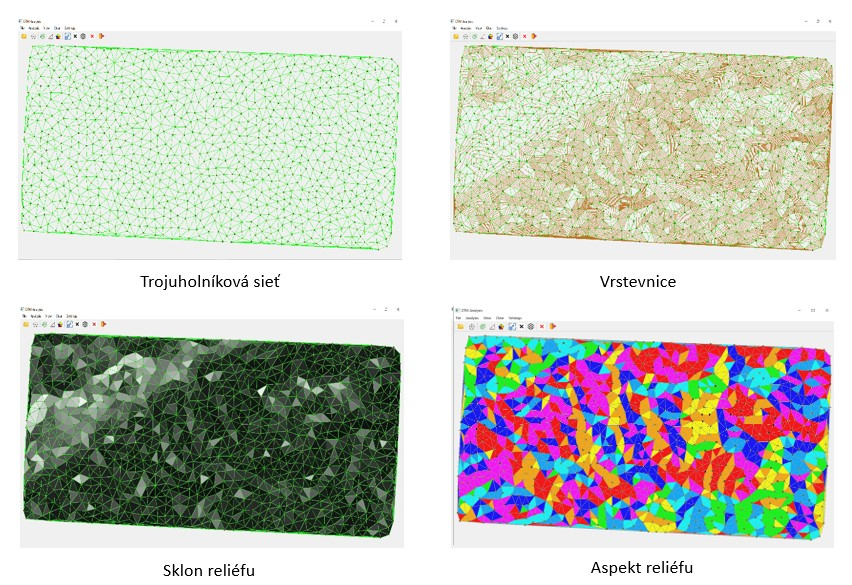
\includegraphics[width=1\linewidth]{latex/images/vysledky.jpg}
    \caption{Výsledky analýzy uzemia}
    \label{fig:enter-label}
\end{figure}
\newpage
\subsection*{Vrcholy}
Ako vrchol nášho záujmu sme si vybrali Stoh, ktorý nie je taký ostrý ako Rozsutec, čo by mohlo prispieť k jeho lepšiemu modelovaniu. Ani jeden z bodov sa však nenachádza na jeho vrchole, prípadne v blízkom okolí. Inak môžeme konštatovať, že zvyšok oblasti je dostatočne reprezentovaný bodmi. Vrstevnice s malým krokom (5 m) nemajú pre túto oblasť nemajú dobrú výpovednú hodnotu, pretožu sú až veľmi nahusto pri sebe. Vrstevnice s korokom 10 metrov sú na tom lepšie ale najlepšie výsledky majú vrstevnice s rozostupom 20 metrov. Je na nich možné pekne sledovať chrbát v smere na Chleb a horšie je viditeľný aj chrbát na Rozsutec. Hlavne je tu ale vidieť Stoh, ktorý ma typický kužeľovoytý tvar. Kvôli nedostatku a zlému umiestnený nahodných bodov sa vrchol Stohu prehliada. To sa prejavuje aj pri sklone, ktorý zobrazuje vrchol Stohu ako terén s malým sklonom (riedke vrstevnice). Takýchto podobných miest sa tu prípade vrcholu.

\begin{figure}[h]
    \centering
    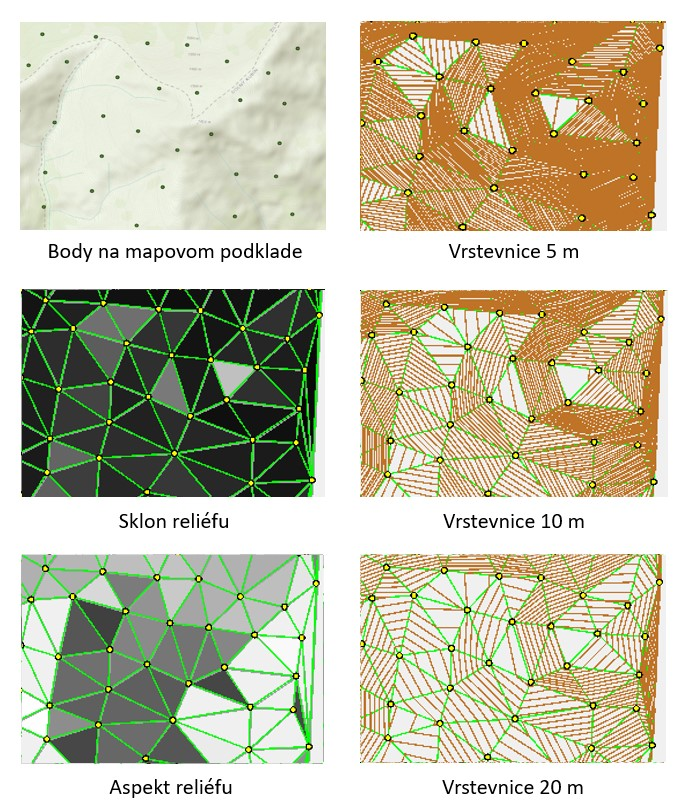
\includegraphics[width=0.6\linewidth]{latex/images/vrchol.jpg}
    \caption{Oblasť s výskytom vrcholu (Stoh)}
    \label{fig:enter-label}
\end{figure}

\subsection*{Hrebene}
Pre túto oblasť bol vybraný hlavný hrebeň Malej Fatry medzi Stohom a Chlebom. Viacero bodov bolo presne vygenerovaných na hrebeni, či v jeho blízkosti. Kedže sa jedná o veľmi strmý svah, tak vrstevnice s krokom 5 a 10 metrev neboli prehľadné a zlievali sa dokopy. Vrstevnice s rozostupom 20 meterov sú oveľa prehľadnejšie a vhodnejšie pre analýzu reliéfu. V čast hrebeňa smerujúca nadol nie je správne reprezentovaná vytvorenými bodmi, ktoré sa nevytvorili v jeho vrchole, ale iba v jeho okolí. To malo za následok, že celý hrebeň v tejto časti bol prehliadnutý, čo sa prejavilo väčším rozostupom vrstevníc. Možeme tak miesto miesto ostrého hrebeňa sledovať relatívne plochý povrch (výrazne menšie prevýšenie), ktorý je obklopený strmým svahom z oboch jeho strán. Potvrdzuje to aj analýza sklonu reliéfu, ktorá tiež poukazuje na tieto miesta. Aspekt reliéfu je veľmi dobre pozorovateľný hlavne v časti hrebeňu smerujúceho na juh. Okrem toho môžeme sledovať aj zmenu orientácie v Šutovskej doline.  

\begin{figure}[h]
    \centering
    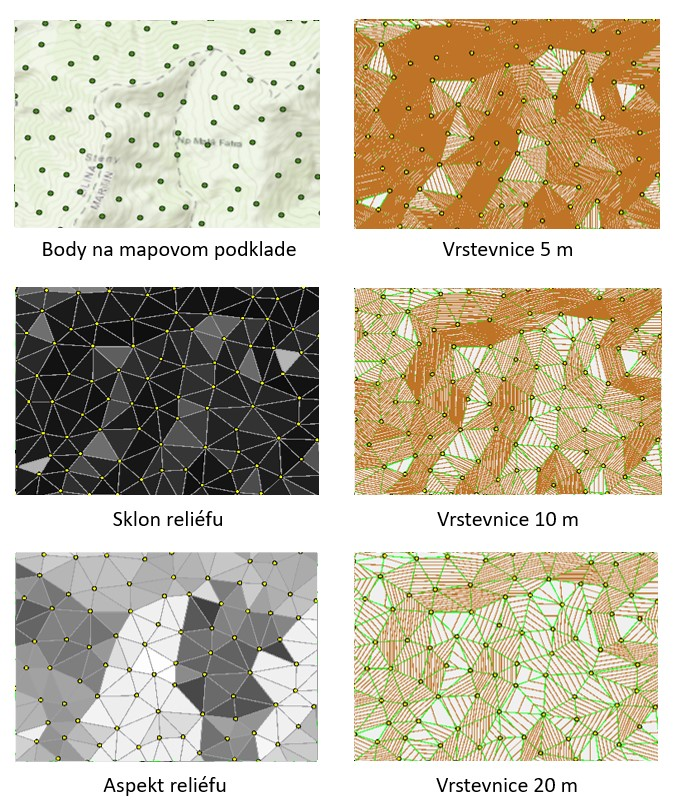
\includegraphics[width=0.56\linewidth]{latex/images/chrbat.jpg}
    \caption{Oblasť s výskytom hreneňa}
    \label{fig:enter-label}
\end{figure}
\newpage
\subsection*{Doliny}
Pri oblasti dolín sme sa zamerali na časť Vrátnej doliny. Nahodné body sa tu vygenerovali na správnych miestach, čiže na dne doliny. Avšak nie všetky body v oblasti mali takýto charakter. Pri triangulácii vznikali miesta, ktoré sa javili ako ploché (s malým sklonom), aj keď podľa mapy sa tam nachádza konkávno-konkávna forma reliéfu. Takýchto prípadov je na tomto území viacero. Pri použití rozličných krokov generovania vrstevníc vyduádza najlepšie výsledok s rozostupom 20 m. Je tu zreteľne vydieť dno doliny aj s priľahlím okolím (menšia členitosť). Pri ďalších dvoch krokoch vrstevníc nie je zreteľné dno doliny, čo je zapríčinené hlavne sklonom okolitého reliéfu, čo súvisý s hustými a neprehľadnými vrstevnicami. Vďaka správnemu vygenerovaniu bodov na samom dne doliny je zreteľne odlíšiteľný aspekt tejto doliny. Pri sklone reliéfu sledujeme zhodu s hustotou vrstevníc. 

\begin{figure}[h]
    \centering
    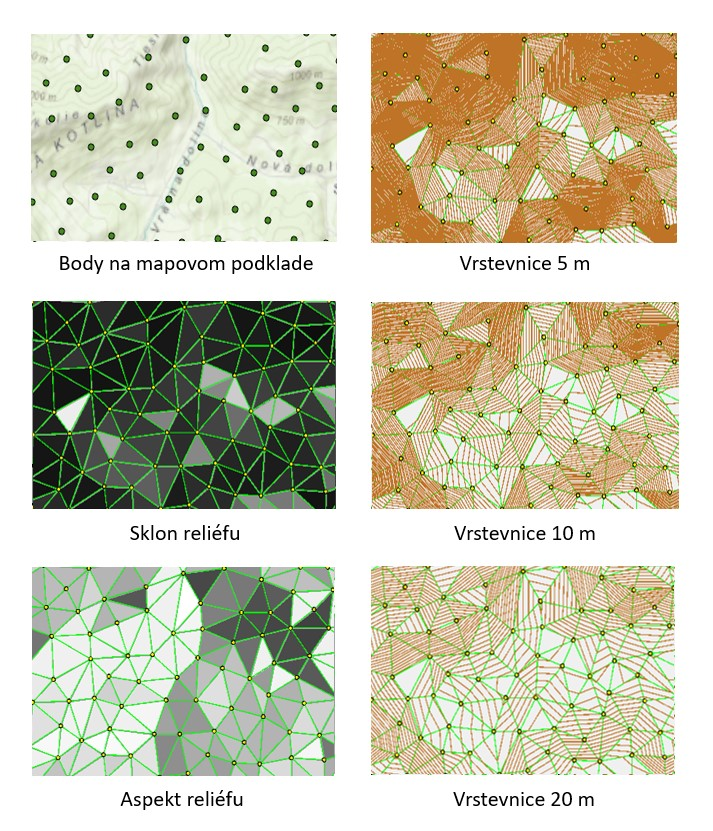
\includegraphics[width=0.6\linewidth]{latex/images/dolina.jpg}
    \caption{Oblasť s výskytom doliny}
    \label{fig:enter-label}
\end{figure}

\subsection*{Rovinaté oblasti}
V okolí obce Dolná Tížina bola najmenšia vertikálna členitosť terénu a oproti zvyšku hornatého územia sa zdala byť relatívne plochá. Rozmiestnenie náhodných dobov sa javia byť podľa vrstevnác správne a vyhovujúce našim potrebám. Z troch rôznych vytvorených vrstevníc sa tie s rozostupom 5 metrov nejavia byť veľmi čitaneľné, na rozdiel od ďalších dvoch krokov. Pri porovnaní týchto dvoch vrstevníc si môžeme všimnúť, že rozostup 20 metrov medzi vrstevnicami je príliš veľký a pre oblasť lepšie opisujú vrstevnice s rozostupom 10 metrov. Na rozdiel od ostatných oblastí je tu oveľa pestrejší sklon reliéfu, kedy sa nejedná iba o strmé svahy. Vďaka tomu je táto oblast pri pohľade na celé naže územie zreteľne odlíšiteľná od hornatých častí. Pri orientácii je zase clé uzemie prevažne orientované iba na jednu stranu, čo pri predchádzajúcich oblastiach bolo práve naopak.  
\begin{figure}[h]
    \centering
    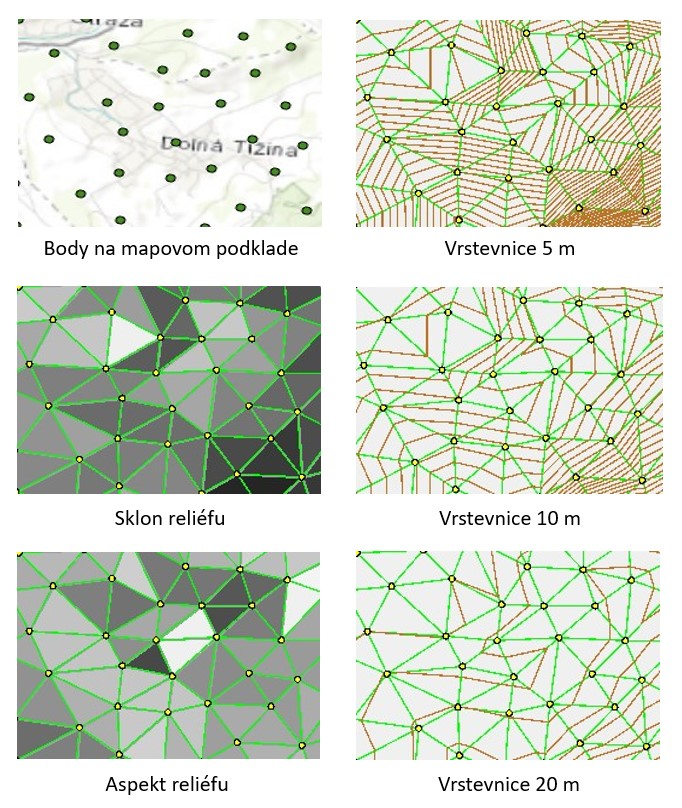
\includegraphics[width=0.6\linewidth]{latex/images/plocha.jpg}
    \caption{Oblasť s menšou vertikálnou členitosťou}
    \label{fig:enter-label}
\end{figure}
\subsection*{Zhodnotenie}
Presnosť celého modelu závisí od hustoty trojuholníkovej siete. Čím zložitejší terén, tým by mala byť hustejšia sieť trojuholníkov. Pokiaľ ku tomu nedôjde, tak môže dôjsť ku výraznému skresleniu v dôsledku vertikálnych a horizontálnych členitostí reliéfu. Napríklad pokiaľ by sa vrchol nachádza uprastred trojuholníku, ktorého body sú v približne rovnakej výške, tak pri vytvorení vrstevníc sa vrchol môže správať ako rovinná plocha (malý sklon). To isté platí aj pri strmích hrebeňoch a kotloch, ktoré môže byť z rovnakého dôvodu naším modelom prehliadnuté. \par
Pri orientácii reliéfu na svetové strany bolo vo viacerých príkladoch možné zreteľne  sledovať tvar dolín a hrebeňov. To dávalo dobrú predstavu o skutočnom tvare reliéfu. Orientácia reliéfu bolo najlepšie pozorovateľné práve v hornatých oblastiach, kde sa nachádzali ostré línie (doliny a hrebene). Pri plochých oblastiach tento jav nebol až taký výrazný, ale stále bol dobre odlíšiteľný .\par
V čom ale vynikali ploché oblasti, tak bolo znázornenie sklonu reliéfu. Na rozdiel od hornatých oblastí je možné sledovať viacero sklonov, zatiaľ čo hornaté oblasti boli v tomto smere monotónne s veľkým sklonom na takmer celom ich územím. Výnimkou boli iba nezachitené vrcholy a hrebene, čo sa prejavovali nižším sklonom.




\newpage
\section*{Záver}
Úlohou tohto zadanie bolo vytvoriť trojuholníkovú sieť pre následnú analýzu digitálneho modelu terénu. Body pre naše územie boli náhodne vygenerované v počte 1000 a aby nedošlo ku veľkému zhluku týchto bodov, tak im bola nastavená minimálna vzdialenosť 300 metrov. Pri voľbe územia bolo potrebné myslieť na jeho tvar, pretože pokiaľ toto územie namalo aspoň podobný tvar ako okno našej aplikácie, tak funkcia Rescale skreslila naše dáta (pri full screen). \par Pre lepšiu analýzu by bolo dobré do budúcna pouvažovať o vytvorení viacerých modelov pre každú špecifickú oblasť sledovaného územia. Zväčšila by sa tak mierka a analýza by bola oveľa podrobnejšia pri zachovaní toho ístého počtu bodov. Pri súčastnej hustote a rozmiestnení náhodných bodov sa najlepšie vygenerovali ploché územia, ale napríklad aj niektoré doliny a chrbty. Pokiaľ teda chceme modelovať a analyzovať toto územie ako celok, tak je potrebné použiť väčšie množstvo bodov. Vyhneme sa tak chybám  ako napríklad pri hrebeňoch, ostrých vrcholoch, konkáv-konkávnych (KK), či  konkáv-konvexných  (KX ) formách reliéfu.
\newpage
\section*{Zoznam použitej literatúry}
\begin{itemize}
       
    \item BAYER, T. 2008. Algoritmy v digitální kartografii. Praha: Nakladatelství Karolinum, 2008. 252 s. ISBN: 978-80-246-1499-1
    \item BAYER, T. Katedra aplikované geoinformatiky a kartografie. Přírodovědecká fakulta UK, Albertov 6, Praha. 2024. Rovinné triangulace a jejich využití. Prednáška z predmetu: Algoritmy počítačovej kartografie. [online] dostupné na: \\https://web.natur.cuni.cz/\~bayertom/images/courses/Adk/adk5\textunderscore new.pdf 
    \item BRŮHA, L. (2016): DIGITÁLNÍ MODELY TERÉNU, výukový materiál, verze 1.0. PřF UK, Praha. [online] dostupné na: https://www.natur.cuni.cz/geografie/\\geoinformatika-kartografie/ke-stazeni/projekty/moderni-geoinformacni-metody-ve-vyuce-gis-kartografie-a-dpz/digitalni-modely-terenu/
    \item DEKAN, T. 2022. Návod na prácu s digitálnym modelom reliéfu v aplikácii QGIS
    verzia 3.0.[online] dostupné na: https://www.geoportal.sk/files/zbgis/lls/navod-pracu-dmr-qgis.pdf

    \item KUBINSKÝ, D. 2024. Morfometrické charakteristiky v prostredí ArcGis. [online] dostupné na: https://www.dkubinsky.sk/clanok/morfometricke-charakteristiky [cit. 01-06-2024]
    \item LIM, J. and PILESJÖ, P. 2022. Triangulated Irregular Network (TIN) Models. The Geographic Information Science & Technology Body of Knowledge (2nd Quarter 2022 Edition). John P. Wilson (Ed.).  DOI: https://doi.org/10.22224/gistbok/2022.2.7
    \item MAUR, P. 2002. Delaunay triangulation in 3D. Plzeň: Katedra informatiky a výpočtovej techniky, Západočeská univerzita v Plzni; 2002. 55 s. [online] dostupné na: https://otik.zcu.cz/bitstream/11025/21617/1/Maur.pdf \\\\
    \item NORDANSJÖ, A. 2024. What is the difference between a Digital Surface Model (DSM) and a Digital Terrain Model (DTM). [online] dostupné na: https://www.globhe.com/resources-collection/what-is-the-difference-between-a-digital-surface-model-dsm-and-a-digital-terrain-model-dtm [cit. 02-06-2024] 
    \item VANÍČEK, T. Katedra inženýrské informatiky. Stavební fakulta ČVUT, Thákurova 7, Praha. 2010. Triangulace. Prednáška z predmetu: Digitální modelování terénu. [online] dostupné na: https://kix.fsv.cvut.cz/\~vanicek/vyuka\textunderscore z09/Triangulace.ppt 
    \item VANÍČEK, T. 2024. Některé teoretické problémy při konstrukci plátového digitálního modelu terénu. [online] dostupné na: http://www.agris.cz/Content/files/\\main\textunderscore files/61/139303/vanit.pdf 
    
\end{itemize}

\section*{Ďalšie zdroje}
\begin{itemize}
    \item Digitálny model reliéfu 5.0 (DMR 5.0) z leteckého laserového skenovania (LLS): ÚGKK SR
\end{itemize}

\end{document}

